\section{Data: Reddit as a community}

We start with a brief overview of both Reddit and the dataset that we use in this paper, focusing on aspects that directly impact our analyses\footnote{There is more to say about Reddit itself (see \url{https://www.reddit.com/about/ }).}.


\subsection{What is Reddit, briefly}

%% DC 10: Will want a couple of legible screenshots here to help illustrate.
%% DC 15: Ideally we would get these numbers as of the end of the dataset to be more consistent.
Reddit is one of the largest sharing and discussion communities on the Web.  According to Alexa, as of late 2015 Reddit is in the top 15 sites in the U.S. and the top 35 in the world in terms of monthly unique visitors.  It consists of a large number of subreddits (853,000 as of June 21st, 2015\footnote{\url
{http://www.redditblog.com/2015/06/happy-10th-birthday-to-us-celebrating.html }for more numbers on reddit size.}), each of which focuses on a particular purpose.  Many subreddits are primarily about sharing web content from other sites: in ``Pics'', ``News'', ``Funny'', ``Gaming', and many other communities, users (``Redditors'') make ``submissions'' of links posted at other sites that they think are interesting.  In other subreddits, Redditors primarily write text-based ``self-posts'': ``AskReddit'', ``IamA'', ``ShowerThoughts'' are places where people can ask questions and share stories of their own lives.  Generically, we will refer to submissions and text posts as ``submissions''.  

%% DC 10: Sam should choose a precise terminology here and use it throughout, and be clear on every single analysis exactly what is being counted.  We don't want someone being confused, trying to replicate the data, and finding something different because they don't understand what the analysis is.  (We will also want to be super-clear below when we introduce the dataset to talk about any filtering we did, so that people can exactly replicate what we did.)

%% DC 10: Further, this terminology should agree with Reddit's, so that people who are familiar with the community aren't confused. 

Each post can be imagined as the root of a threaded comment tree; in addition to submitting, Redditors can make comments, and vote on both submissions and comments.  Votes are used both to sort comments within a submission and submissions within a subreddit, and also form the basis of ``karma'', a reputation system that essentially tracks how often people upvote a given Redditor's comments and submitted links.  Redditors can also create subreddits and volunteer to moderate them.

We choose Reddit as our target community for a number of reasons.  It has existed since 2005, meaning that there has been ample time for the community to evolve and for differences in user cohorts to appear.  Second, being composed of a number of diverse subreddits allows us to explore questions of how communities diverge over time.  Third, Reddit data are publicly available through an API.

\subsection{The dataset}

Redditor \textit{Stuck\_In\_The\_Matrix} used that API to compile a dataset of almost every publicly available comment \footnote{Available in \url{https://www.reddit.com/r/datasets/comments/3bxlg7/i_have_every_publicly_available_reddit_comment }.} from October 2007 until May 2015.  The dataset is composed of 1.65 billion comments, although due to API call failures, about 350,000 comments were not available.  He also compiled a submissions dataset for the period of October 2007 until December 2014 that was made available for us upon request, containing a total of 114 million submissions.  These datasets contain the JSON data returned by the reddit API for comments and submissions \footnote{A full description of the JSON objects is available at \url{https://github.com/reddit/reddit/wiki/JSON }.}; for our purposes, the main items of interest were the UTC creation date, the username, the subreddit, and for comments, the comment text.

We focus on submissions and comments in the dataset because they have timestamps and can be tied to specific users and subreddits, allowing us to perform our time-based analyses.   In some analyses, we look only at comments; in some, we combine comments and submissions, calling them ``posts''.  We would also like to have looked at voting behavior as a measure of user activity\footnote{This would also give us more insight than usual into lurkers' behavior; we'll return to this in the discussion.}, but individual votes with timestamps and usernames are not available through the API, only the aggregate number of votes that posts receive.

\subsection{Pre-processing the dataset}

To analyze the data, we used Google BigQuery \footnote{\url{https://cloud.google.com/bigquery/ }.}, a big data processing tool that at the time of writing this paper provided free processing for up to 1TB of data for users with a Google account.  Redditor \textit{fhoffa} imported the comments into BigQuery and made them publicly available \footnote{See \url{https://www.reddit.com/r/bigquery/comments/3cej2b/17_billion_reddit_comments_loaded_on_bigquery/ }.}.  We uploaded the submission data ourselves using Google's SDK \footnote{Part of the alpha code in the SDK, ``gcloud alpha bigquery import''.}.
%% DC 15: This footnote I don't understand.

For the analyses in the paper, we did light preprocessing to filter out posts by deleted users, posts with no creation time, and posts by authors with names that follow Reddit's conventions for auto-posting bots. 

%The SQL constraints are shown below.
%
%\begin{verbatim}
%created_utc is not NULL
%and author <> '[deleted]'
%and not right(author, 4) = '_bot'
%and not right(author, 3) = 'Bot'
%and not lower(author) contains 'transcriber'
%and not lower(author) contains 'automoderator'
%\end{verbatim}

We also considered only comment data from October 2007 until December 2014 in order to have a matching period for comments and submissions. After this process, we had a total of 1.17 billion comments and 114 million submissions.

%% DC 15: I like big figures, but we could if needed scale/shrink these more to force page boundaries.  Things will change when the front part of the paper changes as well.
\begin{figure*}[!tb]
\centering
\begin{subfigure}{.49\textwidth}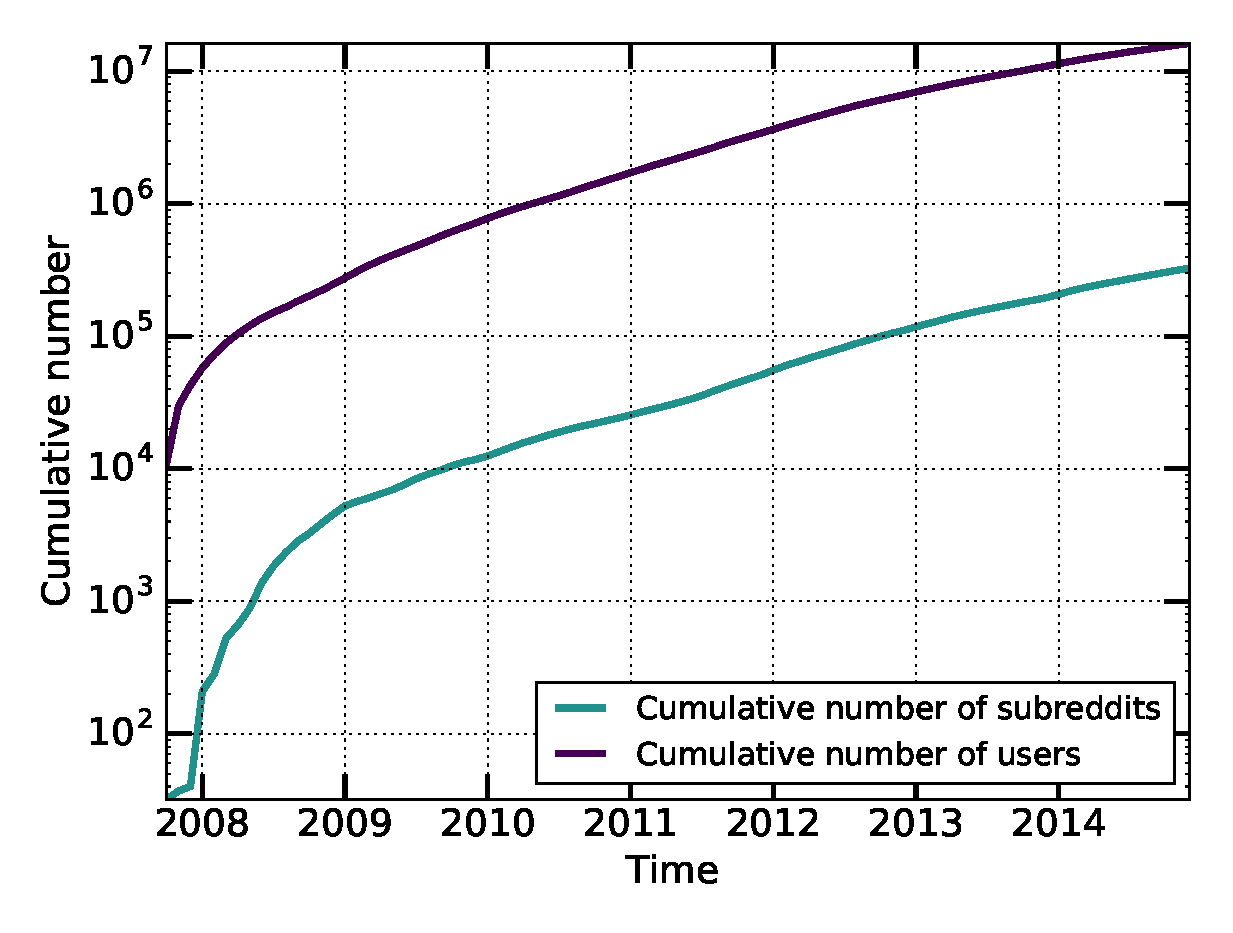
\includegraphics[scale=0.4]{./images/cumulative_users_subreddits.eps}\caption{}\end{subfigure}
\begin{subfigure}{.49\textwidth}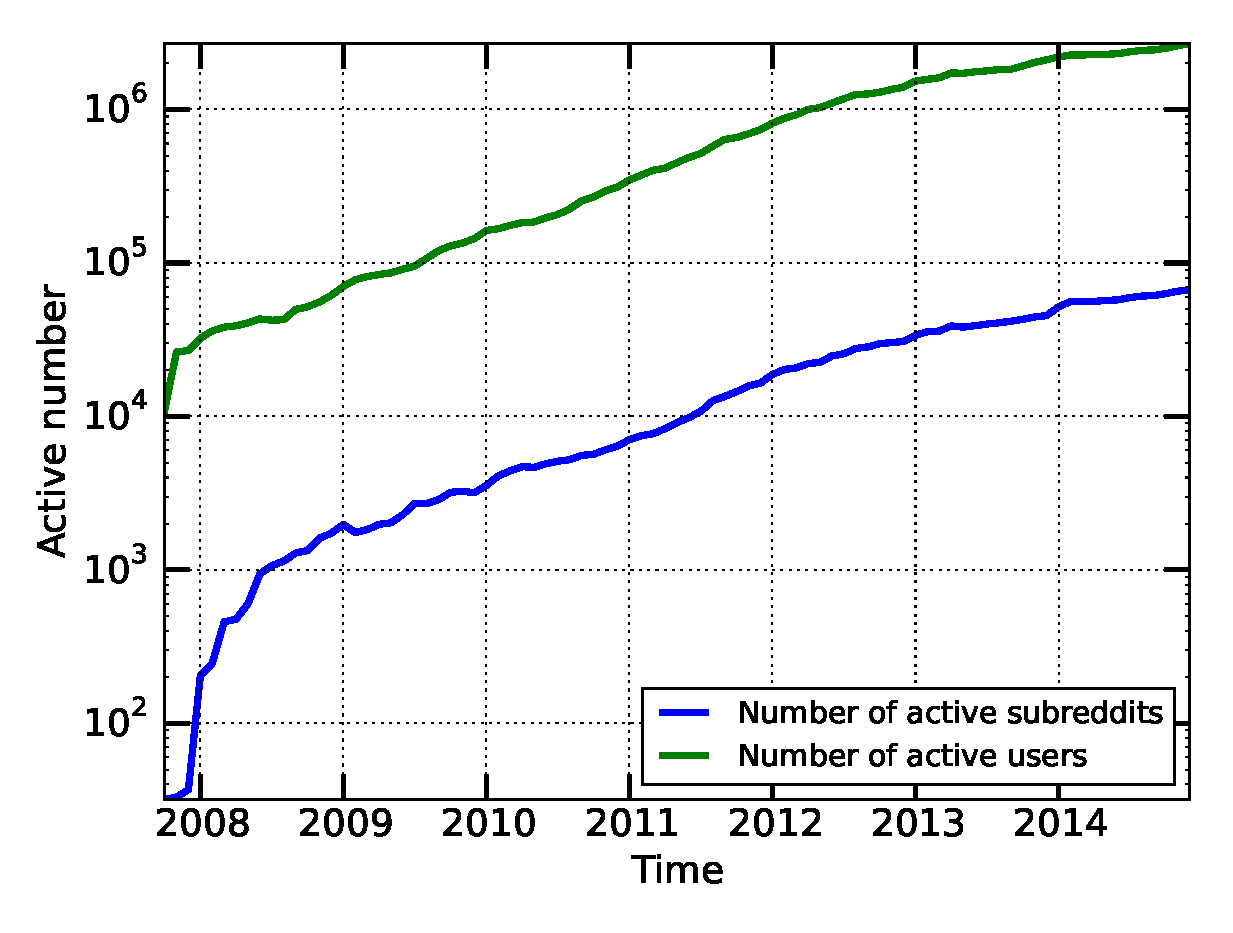
\includegraphics[scale=0.4]{./images/active_users_subreddits.eps}\caption{}\end{subfigure}
\caption{Figure a shows the cumulative growth of reddit for users and subreddits. Figure b shows the number of active users and subreddits in reddit over time. An active user or subreddit is one that had at least one post (comment or submission) in the time bin we used---here, discretized by month.}
\label{fig:cumulative}
\end{figure*}

\subsection{An overview of the dataset}

Here we present an overview of the dataset that shows Reddit's overall growth.  Figure~\ref{fig:cumulative}a presents the cumulative number of user accounts and subreddits created as of the last day of every month. After an initial extremely rapid expansion from 2008--2009, both the number of users and subreddits have grown exponentially.  As of the end of 2014, about 16.2 million distinct users have made at least posts and 327,000 subreddits received at least post since Reddit's inception.

However, as with many other online sites, most users \cite{} and communities \cite{butler_kraut_paper} do not stay active. Figure~\ref{fig:cumulative}b shows the monthly number of active users and subreddits.

We define as an \textit{active user} as one that made at least one post in the month in question. Similarly, an \textit{active subreddit} is one that received at least one post in the month. In December 2014, about 470,000 thousand users and 11,400 subreddits were active, both an order of magnitude less than the cumulative numbers.  

Our interest in this paper is not so much whether users survive as it is about the behavior of active users.  Thus, 
in general our analyses will look only at active users and subreddits in each month; those that are temporarily or permanently gone from Reddit are not included.  

%% DC 15: We don't really look at giving up behavior so much, so, commenting this out.
% The fact that such a significant amount of users stopped using the platform raises questions such as why users give up on their accounts, when they do so, and which users are more likely to stay active. In later sections we will take a closer look at how some of these things are happening in reddit.

\subsection{Identifying cohorts}
%% DC 10: Trying to decide whether this works better here or at the beginning of a cohorty section -- there is some subtlety that I think Sam wants to work through when introducing the first problem.
%% Amit 9: Added this subsection here. Having the cohorts defined as the part of the overview will help, as we talk about them throughout the paper. Some of the cohort stuff from next section can come here. 

We define a user's creation time as the time of the first post by that user or in that subreddit.  Throughout this paper, we will use the notion of user cohorts, which will consist of users created in the same calendar year.

%% DC 15: This is not super-clear, but it is closer.
In many cases, we will look at the evolution of these cohorts. Since users can be created at any time during their cohort year, and our dataset ends in 2014, 
we are likely to have a variation on the data available for each user of up to one year, even though they are in the same cohort.  To deal with this, some of our cohorted analyses will consider only the overlapping time window for which we collect data for all users in a cohort.   This means that we are normally not going to include the 2014 cohort in our analyses.

%% DC 15: Okay, justifying the removal of 2007 is fair enough.
Our data starts in October 2007, but Reddit existed before that. That means that, not only do we have incomplete data for the 2007 year (which compromises this cohort), but there might also be users and subreddits that show up in 2007 that were actually created in the previous years. Since we can not control for these, we will also omit 2007 cohort. We will, however, include 2007 in the overall analyses over time (the non cohorted ones) for two reasons: first, it does not have any direct impact in the results, only extends the axis for 3 extra months, and second, we often compare the cohorted approach with a naive approach based on aggregation, and we would not expect a naive approach to do such filtering. 